\section{Experiment}
\label{sec:experiment}
%\shuqing{Many parts in this section are much more likely to lie in implementation, introducing how \tool works. Doesn't look like experiment.}

%\shuqing{Experiment for devices and case study needed.}

To evaluate the effectiveness of \tool in different modes, we conducted three
experiments on \tool using devices with \ac{USB} Type-C capabilities from different
\acp{OEM}, including a mobile phone, a tablet, and a laptop.

\textbf{Setup.}
%\fengwei{I would suggest to add references for devices such as
%Pi, ATMEGA32U4 board, Yamazawa, etc.}
As mentioned in Section~\ref{sec:badusb},
our \tool only requires common components that are easily accessible online or
in any electronic store. Here we choose the following parts to build a
prototype. To begin with, we choose the Raspberry Pi 4B~\cite{pi4b} as the embedded Single Board
Computer inside \tool, which is powerful enough to process video data and has
an onboard WiFi chip. As for the \ac{HID} Emulator, we use an Atmel ATMEGA32U4 board~\cite{atmel}
with \ac{USB} protocol support, which is able to emulate multiple \acp{HID}
with our modified firmware. About the \ac{USB} 3.x Hub, we use one from the
UGREEN~\cite{ugreen}, which supports HDMI, \ac{USB} 2.0, and many other exported peripherals.
Apart from these essential parts, we also use an auxiliary power bank to
provide power for the Raspberry Pi and the mobile devices used by the victim.
The image of our \tool prototype can be found in Figure~\ref{fig:armory}.

\circled[text=white,fill=myblue]{\scriptsize{A}} is a HUAWEI mobile phone, the victim's device; \circled[text=white,fill=myblue]{\scriptsize{B}} is a compact look of \tool prototype; \circled[text=white,fill=myblue]{\scriptsize{1}} is the \ac{USB} 3.x Hub; \circled[text=white,fill=myblue]{\scriptsize{2}} is a Raspberry Pi 4B as the Single Board Computer; \circled[text=white,fill=myblue]{\scriptsize{3}} is an auxiliary power bank; \circled[text=white,fill=myblue]{\scriptsize{4}} is the Video Capture Card; \circled[text=white,fill=myblue]{\scriptsize{5}} is an Atmel ATMEGA32U4 board as the \ac{HID} Emulator.
%\fengwei{We need to explain the Figure. What is "A"? What is "B", Where are 1,
%2, 3, 4, and 5?}\hongyi{Is the caption sufficient? If explain here, I feel quite redundant}
%\fengwei{I think it is necessary to explain them in the text again.}


\begin{figure}[t]
	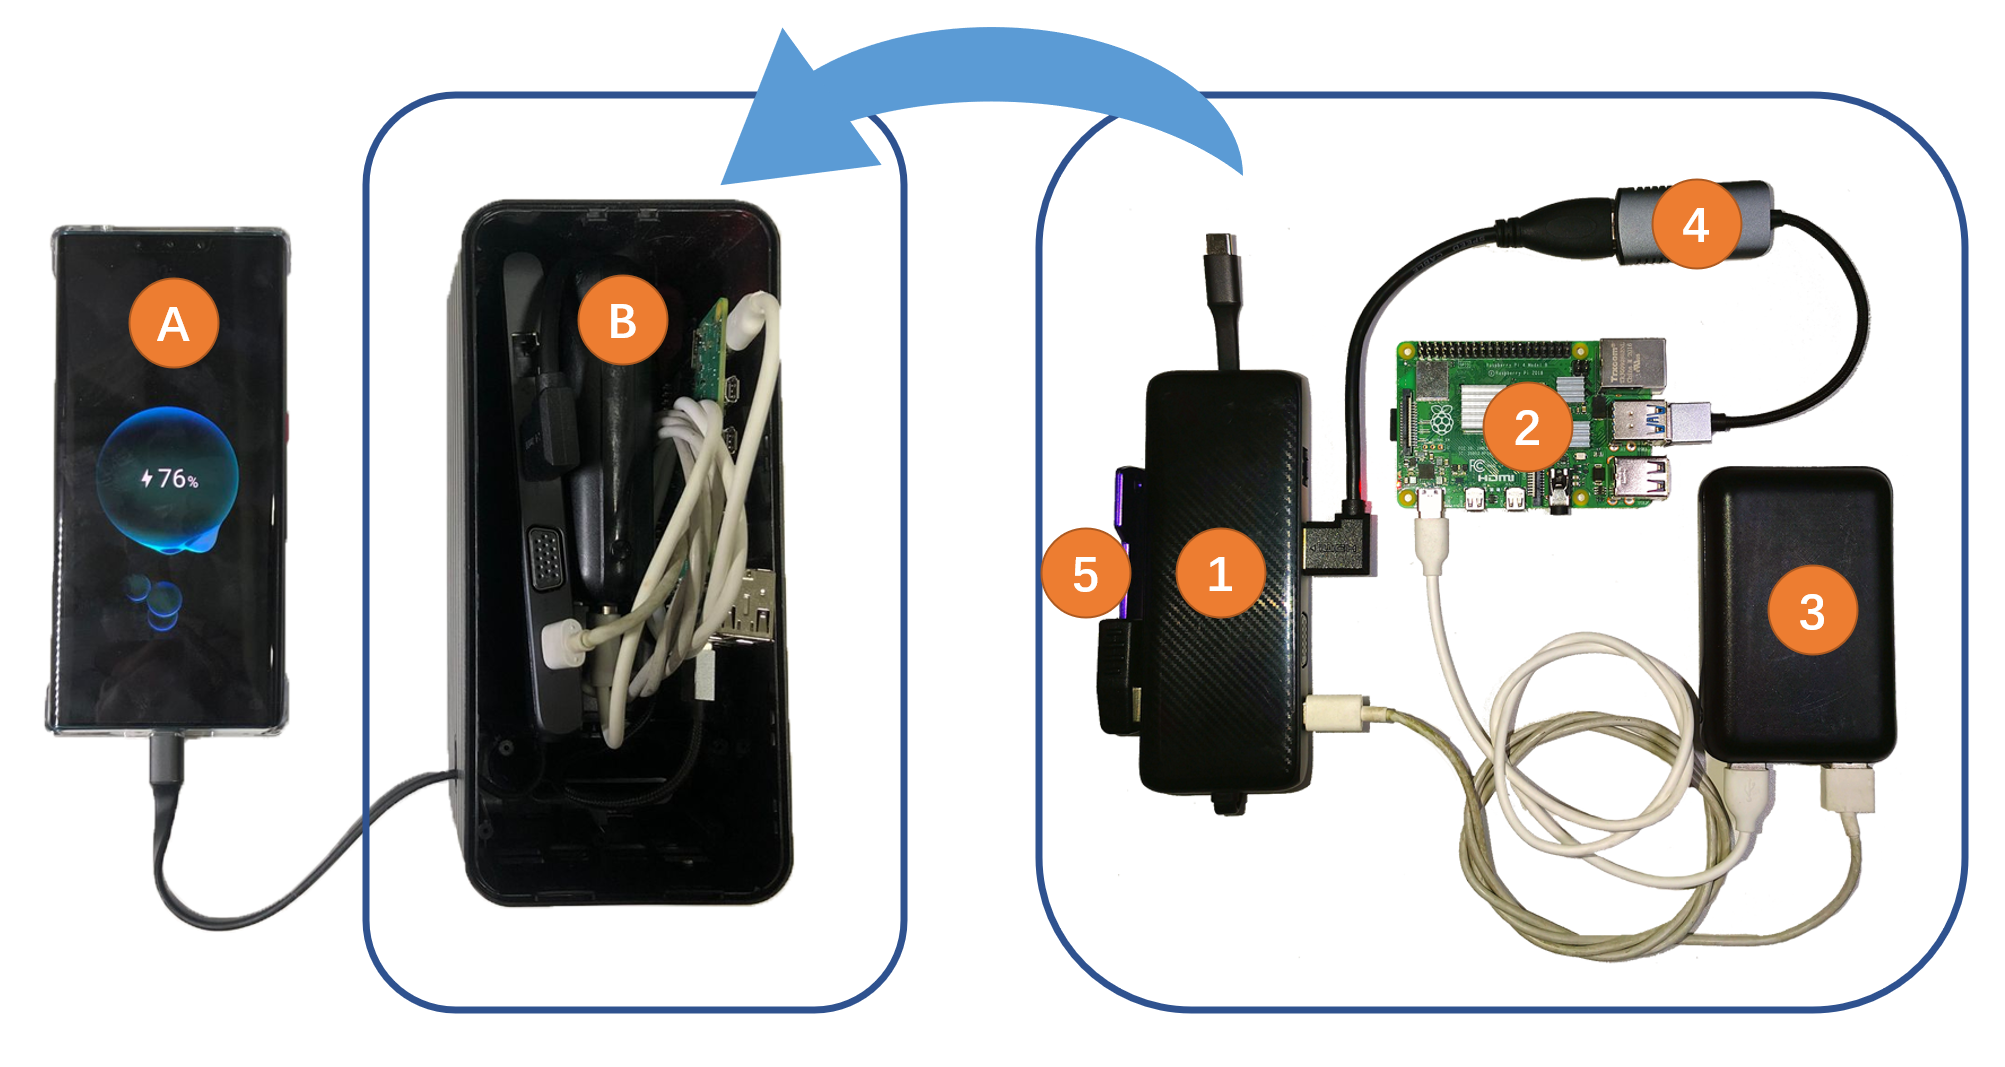
\includegraphics[width=\linewidth]{./Figs/armory_all.png}\\
	\begin{tabular}{ll}
	\circled[text=white,fill=myblue]{\scriptsize{A}} Victim's Device    &\circled[text=white,fill=myblue]{\scriptsize{B}}~\tool\\
	\circled[text=white,fill=myblue]{\footnotesize{1}} \ac{USB} 3.x Hub        &\circled[text=white,fill=myblue]{\footnotesize{2}} Raspberry Pi 4B\\
	\circled[text=white,fill=myblue]{\footnotesize{3}} Auxiliary Power Bank &\circled[text=white,fill=myblue]{\footnotesize{4}} Video Capture\\
	\circled[text=white,fill=myblue]{\footnotesize{5}} ATMEGAA32U4 Board
	\end{tabular}


	\caption{\tool Prototype.}
	\label{fig:armory}
\end{figure}

\subsection{Attack Initialization}
\label{subsec:attack_init}
After the \tool is plugged into the victim's device, there is an initialization process to make sure the \tool is able to carry out subsequent attack.
\begin{itemize}
	\item \textbf{Screen Mirror}:
		During our experiment, we noticed that some devices did not mirror their screens to our \tool by default. In this case, \tool would inject a sequence of keystrokes to set the victim's device into mirror their screens. In both Windows 10 and Ubuntu (Gnome Desktop), \tool can inject `Win+P' (`Super' is another name for the `Win' key) to switch between different modes for external display. Figure~\ref{fig:ubuntu_switch} illustrates how these keystrokes works on Ubuntu and Windows 10 is similar. In MacOS, according to the official manual~\cite{appleman}, \tool can inject \mbox{`Command+F1'} keystroke to set the monitor into mirroring the primary screen. In EMUI, there is a special mode called `Desktop Mode', which allows users to use their smartphones like a desktop computer with an external screen. If this mode is victim's default setting, \tool can inject mouse movements to switch to mirror mode as \tool can obtain victim's `desktop' in this mode.
		\begin{figure}[H]
			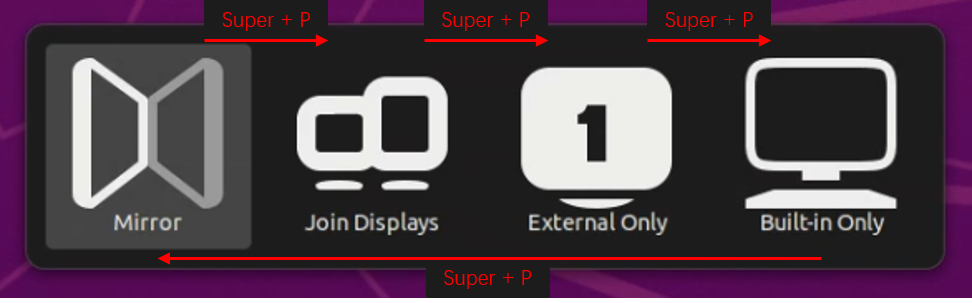
\includegraphics[width=\linewidth]{./Figs/ubuntu_switch.png}\\
			\caption{Screen Mode Switch in Ubuntu.}
			\label{fig:ubuntu_switch}
		\end{figure}
	\item \textbf{Dismiss Notification}:
		In our experiment, we found that some devices will notify the user the presence of an external screen. During our experiment, the following notifications were raised:
		\begin{itemize}
		 \item On Lenovo Xiaoxin Pro 13, it raised a pop-up asking user to select the functionality of the external screen.
		 \item On HUAWEI P30, it showed a status bar indicator and a persistent notification about the external monitor.
		 \item On iPad Pro (the third generation), it also showed a blue status bar indicator and a notification about \ac{USB} accessories if iPad is locked.
		\end{itemize}
		To avoid being discovered by the victim, \tool can inject keystrokes and mouse movements to dismiss some of these notifications. For example, in the first case, \tool is able to inject a sequence of mouse movements to set the screen at mirror mode to dismiss the pop-up.
\end{itemize}
\begin{comment}
\begin{table*}[]
	\begin{tabular}{|c|c|c|c|}
		\hline
		Device                                                               & Operating System                                                                                         & Notification              & Dismiss Action                                            \\ \hline
		\begin{tabular}[c]{@{}c@{}}Lenovo Xiaoxin Pro 13\\ 2020\end{tabular} & Windows 10 (OS Build 18363.1379)                                                                         & Pop-up                    & ``Win+P''-\textgreater{}Mouse click on `Duplicate' Option \\ \hline
		\multirow{2}{*}{HUAWEI P30 (ELE-AL00)}                               & \multirow{2}{*}{\begin{tabular}[c]{@{}c@{}}EMUI 11.0.0.135(C00E128R2P5)\\ Android 10 based\end{tabular}} & Status bar indicator      & N/A                                                       \\ \cline{3-4}
		&                                                                                                          & Persistent notifications  & N/A                                                       \\ \hline
		\multirow{2}{*}{iPad Pro (3rd generation)}                           & \multirow{2}{*}{iOS 14.4 (Build 18D52)}                                                                  & Status bar indicator      & N/A                                                       \\ \cline{3-4}
		&                                                                                                          & Pop-up (only when locked) & N/A                                                       \\ \hline
	\end{tabular}
	\linebreak
	\caption{Notifications about \tool}
	\label{tab:notification}
\end{table*}
\end{comment}

\subsection{HID Emulator Mode}

In the experiment of HID emulator mode, we used {Lenovo Xiaoxin Pro 13
2020}, a PC in Windows 10 \mbox{(OS Build 18363.1379)} and Ubuntu 20.04.2 LTS with two \ac{USB} Type-C interfaces as the
target device. During this experiment, \tool disguised itself as a normal keyboard and an external screen as feedback channel. When first plugged in, the victim's devices raised a pop-up window asking victims what mode should the new screen be set to. \tool immediately injected a sequence of mouse movements and clicks to set itself as a mirror to the primary monitor. Thus we had successfully completed the attack initialization. Then we tested three scripts, ranging from reverse shell backdoor to malware payload execution, all of which resulted in success. Compared to original BadUSB attacks like Rubber Ducky, our \tool can provide attackers real-time feedback which allows attackers to perform more accurate attacks.
%This also warned us that we need more thorough defense against such BadUSB
%attack.


%\fengwei{do we need a reference for OCR?}
%\hongyi{we have discussed this and decide no need.}
\subsection{Video Capture Mode}

During the experiment of privacy extraction via our video capture mode, we chose \mbox{\textit{HUAWEI P30 (ELE-AL00)}}, a
smartphone in \mbox{EMUI 11.0.0.135(C00E128R2P5)} \mbox{(Android 10.0 based)} with a \ac{USB} Type-C interface, as the
target device. In the privacy extraction experiment, \tool passively captured video
from the victim's device and used \textit{OpenCV} to identify the sensitive
information from the video stream.  When the victim viewed text or photos with
text, \tool used the techniques of \ac{OCR}  to
extract text from corresponding video frames. In this experiment, the attacker
successfully extracted text such as name, address, ID number, and other sensitive
personal information. We also tested the payment code extractor, which enables
an attacker to identify payment code in the video stream and performs transactions
without the password. During our experiment, we noticed that this HUAWEI device supports `Desktop Mode'
for its external screen, which enables user to use their devices like a desktop computer with a external screen.
If \tool is set into this mode, \tool is able to inject mouse movements to set itself into mirroring the primary screen, as we discussed in Section~\ref{subsec:attack_init}.
As this is also a part of our case study, more details about
the extracted sensitive data can be found in Section~\ref{subsec:case_study} and
Table~\ref{table:information_extracted}.

%\fengwei{I don't understand the following sentence. Both modes need to capture
%the video stream. Don't understand why it is more power-efficient.}
%\hongyi{Reasonable, changed to other advantage}
Note that the video capture mode only needs to
process the victim's video stream locally, it does not need to transmit the real-time video back to the attacker, which is useful when the network connection between \tool and the attacker is not stable.
%This mode is useful when there is no stable network connection between \tool and the attacker.

\subsection{Fully Control Mode}
%\fengwei{In BadUSB-C section, remote control model is after privacy extraction mode.}

To test the capability of the full control mode, we chose iPad Pro (3rd
	generation), a tablet in iOS 14.4 (Build 18D52) with a \ac{USB} Type-C interface, as the target
device in this experiment.  Besides disguising as normal \acp{HID} like a
conventional BadUSB~\cite{badusb}, \tool also transmitted real-time video
stream from the target device to the attacker via WiFi.  After establishing the connection, the attacker performed a series of actions to test the capability of
\tool. In the beginning, the attacker accessed the album application on the iPad and
obtained all the photos inside. After that, the attacker sent messages via the victim's
account. At last, the attacker performed a transaction using the
financial application. All of these tests resulted in success.

Through this experiment, we have found that with video transmission and mouse
emulation, \tool extensively expanded the attack capability of BadUSB,
especially in mobile devices. In short, we have achieved the complete hijack of the victim's
device in this experiment.

\subsection{Case study}
\label{subsec:case_study}
\tool can be used in various attack scenarios, ranging from mobile devices to PC devices.
For example, \tool can be attached to the power station, which provides USB 3.x hubs, in the airport to perform attacks.
Most people charge their laptops or smartphones in the power station in emergency, with negligence of security.
In the following paragraphs, we will demonstrate the attack scenarios of \tool using sharing power bank as an example.

\subsubsection{Background}

We first introduce the technical background of our case study, sharing power
banks and QR code payment.

\textbf{Sharing Power Banks}.  Sharing power banks provide users with short-term
rental of power banks.  The company deploys power bank stations in the city and
users can rent a power bank from any of the power bank stations, charge their
device on the trip, return the rented power bank to the near stations, and pay
the rental fee.

Power bank sharing is a popular service in Asia, power bank stations are deployed
in markets, stores, and even newsstands. For example, Figure~\ref{fig:PBS_products} are photos
of two power bank stations in China, which are taken outside of a supermarket. Brick~\cite{Brick} is also such a power bank sharing service provider from
Sweden. It provides power bank rental service all over Sweden and is planning on expanding its
service to entire Europe.
\begin{figure}[t]
	\centering
	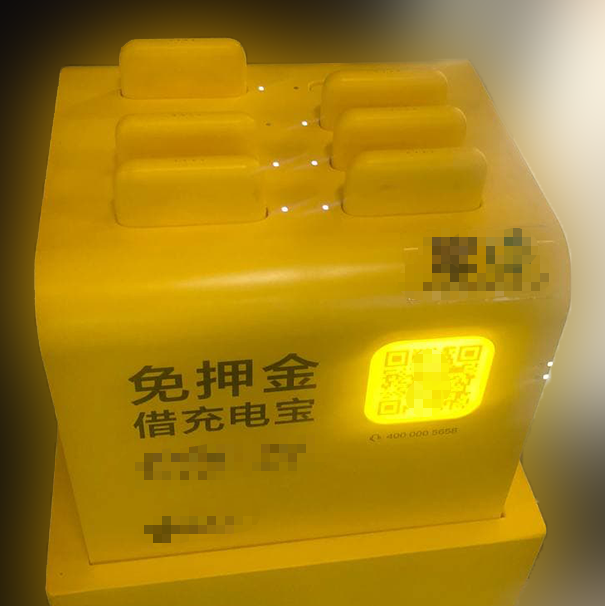
\includegraphics[width=.45 \linewidth, height=.45 \linewidth]{./Figs/PBS_mt.png}
	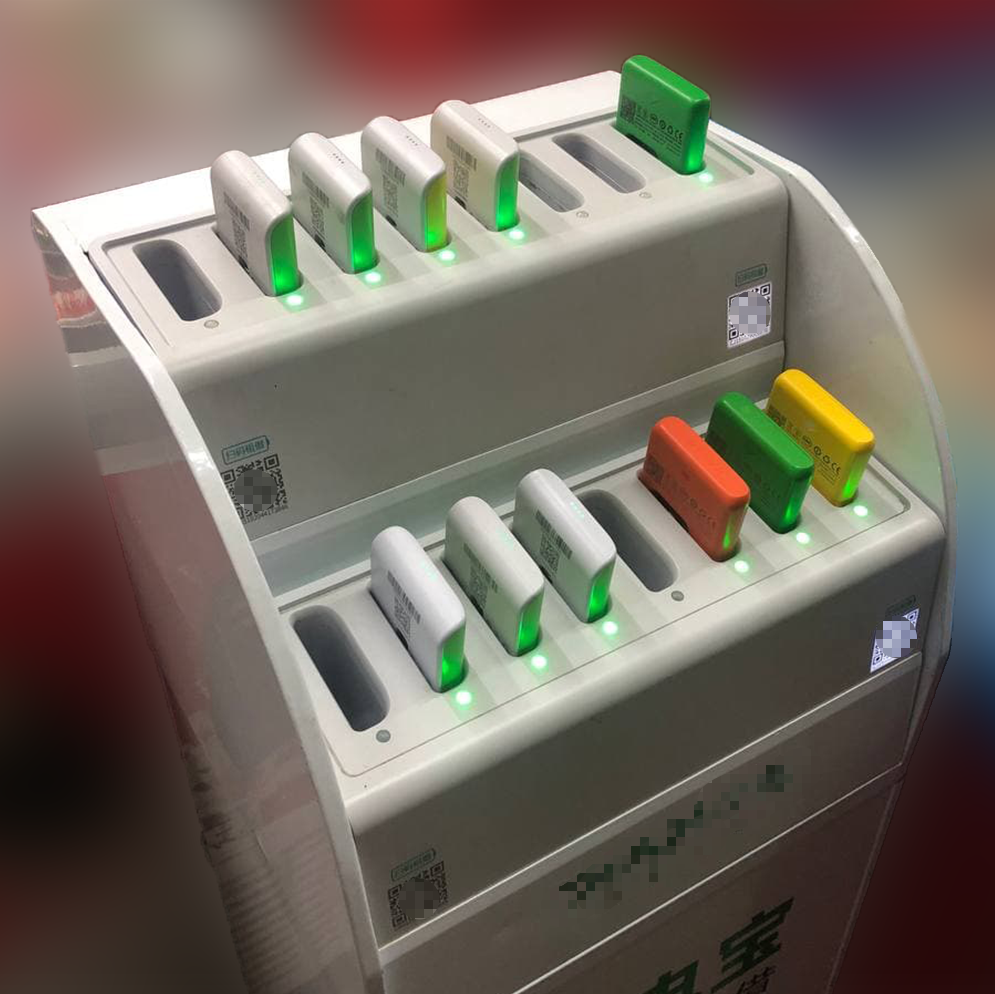
\includegraphics[width=.45 \linewidth, height=.45 \linewidth]{./Figs/PBS_xd.png}
	\caption{Two Power Bank Stations.}
	\label{fig:PBS_products}
\end{figure}

\shuqing{May use statistics (instead of concrete examples) to explain it.}

Sharing power banks not only provides convenience to users, but also brings security issues.  We noticed that most of the power bank stations do not
check the integrity of power banks during the rental process, and users are
hardly cautious to check the power banks when connecting their devices.  An
attacker is able to tamper rented power banks and return them to a power bank
station causing a potential threat to subsequent users.


\textbf{QR Code Payment}.
QR code payment is a new type of payment method that is popular in Asia. Its most well-known cases are WeChat Pay~\cite{Wechat-pay} and Alipay~\cite{AliPay}. QR code payment provides merchant and client a convenient way of offline payment while ensuring equivalent security as the credit card.
As illustrated in Figure~\ref{fig:qr_payment_procedure},
 QR code payments are typically performed in the following steps:
\ding{182} The client presents the payment QR code on the mobile device to the merchant.
The QR code is encoded with a globally unique ID to identify the client's account.
\ding{183} The merchant scans the payment QR code and charges the corresponding amount of money.
By presenting this QR code, the client authorizes the proceeding transaction.
\ding{184} After confirmation, the payment service provider proceeds with this transaction and returns the payment result to both the merchant and the client.
\shuqing{I think this paragraph can be shorter. No need to explain so many details.}
\hongyi{Dont know how to be more concise.}

\begin{figure}[t]
	\centering
	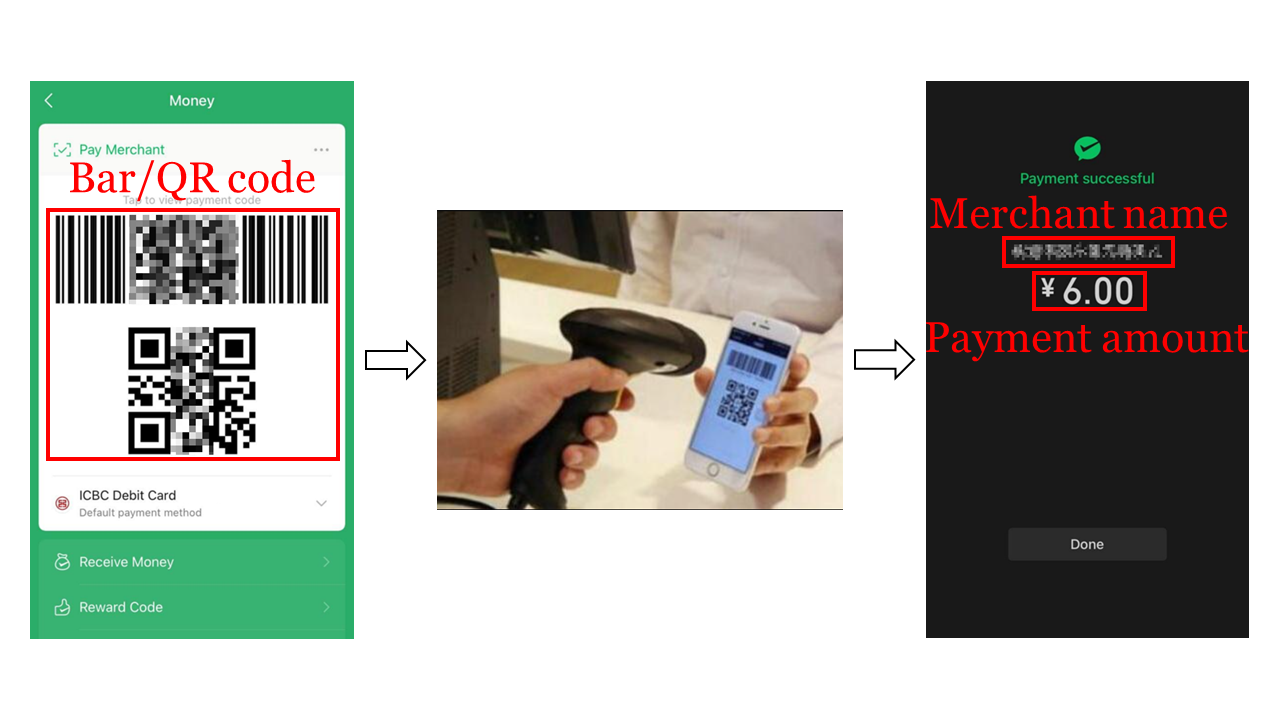
\includegraphics[width=\linewidth]{./Figs/qr_code_payment.png}
	\caption{Bar/QR Code Payment Procedure.}
	\label{fig:qr_payment_procedure}
\end{figure}


Next, we explain one type of payments called micropayment. A micropayment is pre-determined by the payment
service provider with thresholds in the user agreement. In real-world scenarios, payment service providers use different rules
for micropayment purchases. For example, WeChat
Pay~\cite{Wechat-pay} regards transactions under USD \textdollar 154 as
micropayments.  Different from a typical payment procedure, when micropayments
are made, confirmations can be applied automatically without clients'
permission which aims to provide convenience to both merchant and client.  If a
victim's payment code is leaked to the attackers, they can use that code to
authorize multiple micropayments without needing permission.  In order to prevent such
cases, both WeChat Pay~\cite{Wechat-pay} and Alipay~\cite{AliPay} have designed a refreshing mechanism for the
payment code, which is to refresh the QR code every minute. This is sufficient
to stop an attack like opportunistic theft of a payment code but unable to stop a real-time attack like our
\tool.  In summary, the payment QR code is highly sensitive on users' devices
and our following case study is about how to obtain this code using an
attacker-crafted power bank via \tool.

\subsubsection{Attack Scenario}

In this part, we will introduce a real-life attack scenario to show that our
\tool is a practical offensive tool.  This scenario can be broken down into the
following steps.

\begin{enumerate}[I. ]
	\item The attacker rents a power bank from one of the power bank stations and replaces the internal components with \tool.
	\item After the modification, an attacker-crafted power bank is returned to a rental station in a crowded area like an airport or railway station, which increases the probability of success.
	\item A user borrows the modified power bank and connects it to his/her own device, becoming the victim of \tool.
	\item The attacker now has complete control over the victim's device and can perform various attacks using different modes.
\end{enumerate}

Next, we summarize the possible threats toward users under different modes.
%\hongyi{Better way to express this?}
First, under \ac{HID} emulator mode, the attacker is able to implant malware and backdoor scripts into victims' devices. Moreover, using video capture mode, once the victims access their sensitive data such as QR payment  code or photos, their sensitive data will be immediately transmitted via \tool to the attacker. Lastly, with full control mode, the attacker has complete control over the victims' device and can conduct any action on the victim device.

\shuqing{Background is longer than real user study.}
%As the functionality and effectiveness, HID emulator mode is similar to the original BadUSB and the full control mode hijacks the victim's device completely.
\hongyi{I dont know if it's a good enough reason}
%Here we only validate the usability of privacy extraction mode and conducted a user study.


We notice that, with \tool, the attacker can view any victim's information that does not require authentication with video capture mode or full control mode.
However, the information that requires authentication can only be obtained with video capture mode after the victim's authentication.
To further validate our attacking scenario, we conduct an experiment to find out what types of sensitive information are protected by default. We installed x applications on an Android phone, set up each application with the strategy that
\ding{182} Login in with a test account,
\ding{183} Keep the default settings,
\ding{184} Agree to it when it asks to enable authentication before accessing private data, then
recorded all information shown in applications with or without authentication. The result is shown in the Table~\ref{table:information_extracted}.

However, if the victim uses a password instead of biometric authentication, the password can be leaked out and cause greater harm, such as guessing other passwords on the device.
As the victim uses the device and accesses information, the possibility of the leakage of information that needs authentication would increase, and this kind of information often brings greater risk such as hacking accounts.
Meanwhile, the leakage of the information that can be obtained without authentication is enough to bring potential risk to the victim, such as misappropriating the victim's payment code, using the victim's personal information for illegal crimes.


\subsubsection{Result}

In summary, though we cannot directly obtain the user's password on the lock screen, we can still check all of the information presented on the screen, extract sensitive information including but not limited to social accounts, bank accounts, personal financial situation, if the user unconsciously unlocks the screen.
The information that requires authentication is still safer than the information that does not require authentication. The attacker can not directly obtain this kind of information aggressively through the full control mode.
It is worth mentioning that {secure keyboards} built in financial apps show their keyboard typing sequences, which can be easily captured by \tool.



\begin{table*}[t]
	\centering
	\begin{tabular}{|c|c|c|c|c|c|}
		\hline
		\textbf{Category}  					& \textbf{Application} & \textbf{Leaked Sensitive Information}		& \textbf{Leaked Sensitive Information after Authentication} \\
		\hline
		Social \& Finance App 				& WeChat      & WeChat account, Asset status, chat history    		& \\
		\hline
		\multirow{3}{*}{Social App}			& QQ          & QQ account, interpersonal nexus, chat history   	& \\
											\cline{2-4}
							       			& Twitter     & Twitter account, interpersonal nexus            	& \\
											\cline{2-4}
							       			& Gmail       & Gmail account, Mail records                     	& \\
		\hline
		\multirow{3}{*}{Finance App}       	& Alipay      & Alipay account, Asset status         				& \\
											\cline{2-4}
											& ICBC        & ICBC account, password, Asset status  				& \\
											\cline{2-4}
											& Paypal      & Paypal account, bank accounts, Asset status     	& \\
		\hline
		\multirow{2}{*}{Tool}               & Chrome      & Sites visited                                   	& \\
											\cline{2-4}
		                					& Health      & Personal physical metrics      						& \\
		\hline
		\multirow{2}{*}{System}             & Settings - WiFi   & WiFi SSID                                	&  WiFi password \\
											\cline{2-4}
		                					& Settings - VPN    & VPN address, VPN account, VPN password      						& \\
		\hline
	\end{tabular}
	\linebreak
	\caption{Information Extraction via Manual Analysis.}
	\label{table:information_extracted}
\end{table*}



%%%%%%%%%%%%%%%%%%%%%%%%%%%%%%%%%%%%%%%%%%%%%%%%%%%%%%%%%%%%%%%%%%%%%%%%%%%%%%%%%%%%%%%%
% It is unfortunate that the user study is not part of the paper anymore.
\iffalse

To further validate our attacking scenario, we invited 10 volunteers, who are students in our university, to participate and conduct a user study.
Before the user study experiment, we disclosed to the volunteers how their data might be used and request permission from the volunteers and the university ethics review boards.
During the case study, volunteers took turns to use their phones for half an hour with \tool connected.
To obtain data close to real-life, they were requested to use phones just as they were normally using sharing power banks.
At the same time, we used scripts to perform \ac{OCR} recognition for each frame in the videos stream and stored all of the \ac{OCR} results in a database.

After each experiment, the raw video and the corresponding \ac{OCR} result file was generated automatically, then we presented these files to him/her, introduced our attack, told him/her to analyze the video file and replace certain characters of the private data that appear in the \ac{OCR} result file with asterisks. This protects their privacy and is also a mark for us to confirm that the data we find contains their private data. At last, he/she would destroy all original files, leave only the desensitized \ac{OCR} results for us.
%\shuqing{Do we need to mention that agreement the conference required here?}
%\hongyi{I'm also quite concern about this.}


\subsubsection{Result}

In total, there are 94,058 entries of data from 10 volunteers. An entry is a combination of the case number, the frame number and the desensitized \ac{OCR} result.
%\shuqing{The data may need to be updated.}
With these results, we could learn what content the victim visited, especially the privacy data.
%\fengwei{The following text needs to be revised. It is quite difficult for me to understand. Note that this is important text because reviewers are curious about the result. }
We searched the result database with the keywords \textit{account, username, password, phone number and email}, as well as the regular expression of email.
The records searched by such keywords and regular expressions are usually related to privacy information of users.
For example, when we searched with \textit{account} as a keyword, victim's accounts could be found in the database, as shown in the Table~\ref{tab:ocr_keyword_example} and Table~\ref{table:information_extracted}.
%\shuqing{Statistics.}
At last, we found 4,172 of 94,058 records obtained by \tool which are related to privacy information, as shown in the Table~\ref{table:information_extracted}.

In summary, though we cannot directly obtain the user's password on the lock screen, we can still check all of the information presented on the screen, extract sensitive information including but not limited to social accounts, bank accounts, personal financial situation, etc., if the user unconsciously unlocks the screen.
It is worth mentioning that {secure keyboards} built in financial apps show their keyboard typing sequences, which can be easily captured by \tool.



\begin{table*}[t]
	\centering
	\begin{tabular}{|l|l|l|l|}
		\hline
		\textbf{Keyword} & \textbf{Text}                                                             & \textbf{Name}                                   & \textbf{Frame Number} \\ \hline
		username                          & X 8B cas.******.edu.cn Username: 11****18 Password:                                        & \textless{}user1\textgreater{} & 385                                    \\ \hline
		username                          & Login Weibo Login with SMS and verification code ...... +86 151****4587                    & \textless{}user5\textgreater{} & 1947                                   \\ \hline
		username                          & QQ 14*****50| Login with phone number New user registration 2345678 9 0                    & \textless{}user3\textgreater{} & 4308                                   \\ \hline
		username                          & connect to *** username h*****l Save account information Open VPN.....                     & \textless{}user6\textgreater{} & 7925                                   \\ \hline
		phone number                      & Login with phone number ...... +86 186****2483 |                                           & \textless{}user1\textgreater{} & 313                                    \\ \hline
		phone number                      & Log in with your mobile phone number. ...... mobile phone number 131****9310 & \textless{}user9\textgreater{} & 210                                    \\ \hline
		@                                 & contact email 30*******7G@qq.com, contact phone 027-88******                               & \textless{}user7\textgreater{} & 5324                                   \\ \hline
		@                                 & Account 73*****5@qq.com @qq.com @163.com @gmail.com 	......      & \textless{}user6\textgreater{} & 621                                    \\ \hline
	\end{tabular}
	\linebreak
	\caption{Examples of Searching \ac{OCR} Results with Keywords.}
	\label{tab:ocr_keyword_example}
\end{table*}

\begin{table*}[t]
	\centering
	\begin{tabular}{|c|c|c|c|c|c|c|}
		\hline
		\textbf{Keyword}                               & Account & Password & Phone number & Email & Username & Regexp for email~  \\
		\hline
		\textbf{Number of records containing keywords} & 680     & 1,596     & 1,510         & 164   & 522      & 78                 \\
		\hline
		\textbf{Total Number of Records} & \multicolumn{6}{c|}{4,172} \\
		\hline
	\end{tabular}
	\linebreak
	\caption{Privacy Extraction Result.}
	\label{table:information_extracted}
\end{table*}

\fi
